\section{Verifikation und Validation}
\subsection{Unterschied zwischen Verifikation und Validation}
Sicherstellen, dass das Softwaresystem die Benutzeranforderungen erfüllt.
\begin{multicols}{2}
    \subsubsection{Verifikation}
    \begin{itemize}
        \item Machen wir das Produkt richtig?
        \item Die Software soll den Anforderungen entsprechen.
    \end{itemize}
    
    \subsubsection{Validation}
    \begin{itemize}
        \item Machen wir das richtige Produkt?
        \item Die Software soll machen, was der Benutzer wirklich benötigt.
    \end{itemize}
\end{multicols}

\begin{multicols}{2}
    \subsection{Qualitätskosten}
    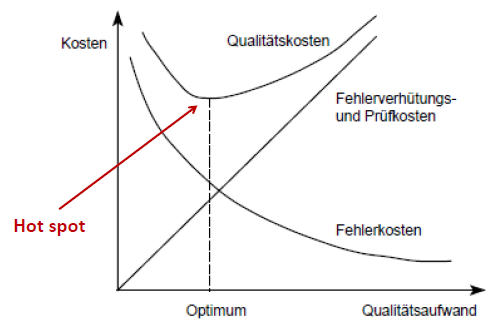
\includegraphics[width=0.48\textwidth]{images/VerifikationValidation/qualitaetskosten}
    
    \subsection{Lebenszyklus}
    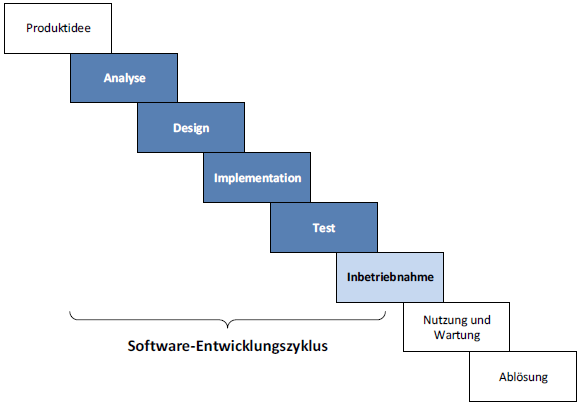
\includegraphics[width=0.42\textwidth]{images/VerifikationValidation/lebenszyklus}
\end{multicols}

\subsection{Tests}
\begin{wrapfigure}[3]{r}{0.5\textwidth}
    \vspace{-12pt}
    \centering
    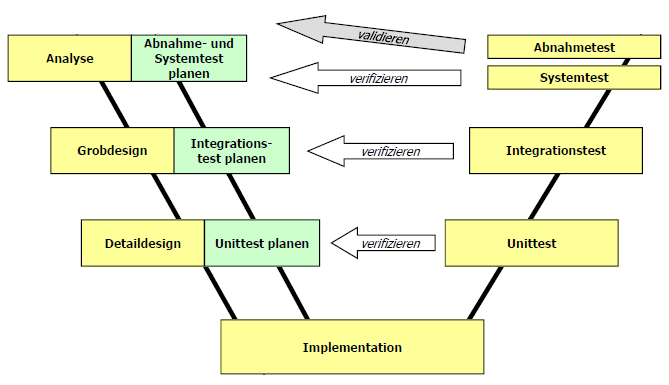
\includegraphics[width=0.48\textwidth]{images/VerifikationValidation/vmodell}
\end{wrapfigure}
\ 
\vspace{-10pt}
\begin{itemize}
	\item Unittest
		\begin{itemize}
			\item Teil der Implementationsphase
			\item Whitebox-Test
			\item Durch Programmierer
		\end{itemize}
	\item Integrationstest
		\begin{itemize}
			\item Zusammenfügen mehrerer Units
			\item Blackbox-Test
			\item Schwerpunkt: Unit-Schnittstellen
			\item Nicht durch Programmierer
		\end{itemize}
	\item Systemtest
		\begin{itemize}
			\item Testen des Gesamtsystems in Originalumgebung
			\item Blackbox-Test
			\item Schwerpunkt: Externes Verhalten des Systems
			\item Nicht durch Programmierer
		\end{itemize}
    \item Abnahmetest
	    \begin{itemize}
		    \item Ziel der oberen Tests: Fehler finden
		    \item Ziel der Abnahmetest: Erfüllung von festgelegten Kriterien für geforderte Funktionen nachweisen 
		    \item wird durch Auftraggeber durchgeführt
	    \end{itemize}
\end{itemize}

 \subsubsection{Prüfverfahren}
 \begin{itemize}
     \item Review (viel zu selten eingesetzt)
     \item Statische Tests (ohne Ausführung des Programms)
     \item Dynamische Tests (durch Ausführung des Programms)
     \item Simulation
     \item Einsatz von Prototypen (kritische Teile werden vorab untersucht)
 \end{itemize}
 
 \subsubsection{Testabschlusskriterien: wann ist das System good enough}
 \begin{itemize}
    \item Wenn alle Testfälle der Testvorschrift erfolgreich durchgeführt worden
sind
        \begin{itemize}
            \item Häufiges Kriterium in der Praxis
            \item Dieses Kriterium ist sinnvoll, wenn eine systematische Auswahl von Testfällen
eine ausreichende \\ Überdeckung ermöglicht
        \end{itemize}
    \item Wenn die Prüfkosten pro entdecktem Fehler eine im voraus festgelegte
Grenze überschreiten
        \begin{itemize}
            \item Sinnvolles Kriterium für das Beenden des Systemtests
            \item Setzt die Erfassung der Prüfkosten und der Anzahl gefundener Fehler voraus
        \end{itemize}
 \end{itemize}
 
 \subsubsection{Infinite faults}
 \begin{itemize}
     \item Ein System hat unendlich viele Fehler (infinite faults) wenn trotz Testen
und Debugging die Fehlerzahl um einen unakzeptabel hohen Wert oszilliert
    \item Kosten für zusätzlich eliminierten Fehler = $\infty$
    \item Massnahme: vernünftigerweise meist nur Projektabbruch
 \end{itemize}

\subsection{Testen von Embedded Systems}
\begin{itemize}
    \item \textbf{Annahme:} Das Embedded System ist vernünftig strukturiert in hardware-abhängige und hardware-unabhängige Teile
    \item \textbf{Hardware-unabhängige Teile:} Die Unittests dieser Teile können auf der Entwicklungsplattform (meist PC) wie übliche PC-Applikationen getestet werden.
    \item \textbf{Hardware-abhängige Teile:} Wenn Units auf externe Hardwaresignale reagieren oder externe Hardwaresignale generieren müssen, so müssen diese durch geeignete Hardware generiert, bzw. konsumiert werden. In diesen Fällen bietet sich externe Testhardware für Driver und Stubs an
\end{itemize}

\subsubsection{Reviews}
\begin{itemize}
    \item Reviews sind die effizienteste Testmethode
    \item Reviews sind öffentliche, verbale Begutachtungen eines erstellten Arbeitspakets.
    \item Reviews sind eine zwischenmenschliche Angelegenheit. Der Erfolg hängt von der persönlichen Dynamik zwischen Autor und Gutachtern ab.
\end{itemize}

\paragraph{Begründung für Reviews}
\begin{itemize}
    \item Fehler finden
        \begin{itemize}
            \item Fehlerursachen finden, nicht nur Symptome
            \item Mit Reviews werden am meisten Fehler gefunden
            \item Kaum reproduzierbare Fehler wie z.B. Synchronisationsfehler bei Multithreading können am besten mit einem Review entdeckt werden
        \end{itemize}
    \item Wissenstransfer
        \begin{itemize}
            \item Alle Beteiligten (Autor und Reviewer) lernen etwas
        \end{itemize}
    \item Wirtschaftlichkeit
        \begin{itemize}
            \item Reviews sind sehr wirtschaftlich
        \end{itemize}
\end{itemize}

\paragraph{Rollen der Beteiligten}
\begin{itemize}
    \item Moderator
        \begin{itemize}
            \item organisiert und leitet
        \end{itemize}
    \item Gutachter (2-3)
        \begin{itemize}
            \item prüfen, nennen Befunde
        \end{itemize}
    \item Autor
        \begin{itemize}
            \item verhält sich passiv, hört zu
            \item erläutert allenfalls (möglichst vermeiden)
            \item protokolliert die Befunde (dadurch erspart man sich einen expliziten Schreiber)
        \end{itemize}
\end{itemize}